\documentclass[conference]{IEEEtran}
\IEEEoverridecommandlockouts
\usepackage{cite}
\usepackage{amsmath,amssymb}
\usepackage{graphicx}
\usepackage{booktabs}
\usepackage{multirow}
\usepackage{xcolor}
\usepackage{url}
\graphicspath{{figures/}}

\newcommand{\best}[1]{\textbf{#1}}

\begin{document}

\title{Vision-Measured Queue Tails for Storage-Aware Adaptive Traffic Signal Control}

\author{\IEEEauthorblockN{Hemang Bhat and Jatin}
\IEEEauthorblockA{Hemang Bhat: 2024UCA1829 \quad Jatin: 2024UCA1865\\
Netaji Subhas University of Technology\\
New Delhi, India}}

\maketitle

\begin{abstract}
Camera-based adaptive signal controllers usually reduce each approach to a vehicle
count. A count does not say where the queue ends, or how much road the approach has
left, which is the quantity that spillback avoidance depends on. We measure the
position of the queue tail directly from a single traffic camera using YOLOv8
detections and ByteTrack identities: a stopped test normalised by each vehicle's own
image size, and a contiguous chain of stopped vehicles followed back from the stop
line along a drawn queue axis. In a cached YOLOv8n measurement audit, stop events fall from 4.28 to 0.76 per vehicle; this measures stability rather than labelled accuracy. We then ask whether this measurement improves control,
using closed-loop simulation in SUMO with protocols fixed before the test runs. Added
as a term in the selection score of a density-based controller, the queue tail gives no statistically significant delay improvement and alters the chosen approach in 1 of 40 inspected runs. Used instead as a storage limit on green time, following the spillback constraint
of Mohajerpoor \emph{et al.}, it reduces blocked-entry time by 20--26\% against actuated
control near capacity without an observed delay penalty, and on a junction with a
short side street it outperforms a count-based version of the same rule. Beyond
capacity the rule increases delay by 81--91\,s. We report both outcomes and the
mechanism behind each.
\end{abstract}

\begin{IEEEkeywords}
adaptive traffic signal control, queue length estimation, object tracking, spillback,
SUMO, YOLO
\end{IEEEkeywords}

\section{Introduction}
A signalised junction repeatedly makes two decisions: which approach receives the next
green, and for how long. Fixed-time plans make both decisions from historical averages.
Actuated and adaptive controllers make them from measurements, traditionally from
inductive loops, which report presence at one point of the road. A camera observes the
whole approach, and recent work replaces loops with a detector network that counts
vehicles per approach~\cite{raza2025}.

A count is a weak description of a queue. Ten vehicles on a 60\,m approach and ten
vehicles on a 150\,m approach give the same count, although the first approach is
almost full. When a queue reaches the upstream end of its link (spillback), arriving
vehicles are blocked and congestion propagates to neighbouring junctions. Controllers
designed for over-saturation therefore constrain the queue \emph{position} relative to
the link length~\cite{mohajerpoor2023}, but they obtain that position from a traffic
flow model driven by predicted demand, because loop detectors cannot observe it.

This paper studies whether a camera can supply that quantity, and whether supplying it
helps. The contributions are:
\begin{itemize}
\item a calibration-free measurement of the queue tail from detections and tracks,
with a perspective-normalised stopped test and a contiguous-chain definition of the
queue (Section~\ref{sec:measure});
\item a controlled negative result: used only to rank approaches, the measurement rarely changes the decisions of a density-based controller, and we explain why
(Section~\ref{sec:study1});
\item a storage-aware rule that uses the measurement as a limit on green time, and an
evaluation against fixed-time, actuated, capacity-aware max pressure and
density-based control over graded demand, including the regime in which the rule
fails (Section~\ref{sec:study2}).
\end{itemize}
All experiments are reproducible from the accompanying repository.\footnote{\url{https://github.com/hemangbhat/CV_Project}}

\section{Related Work}
\subsection{Vision-based signal control}
Raza \emph{et al.}~\cite{raza2025} deploy YOLO detectors on edge devices and convert
detections into a density weighted by passenger car equivalents (PCE),
$D=\sum_c n_c\,\mathrm{PCE}_c$, further scaled by a lane-priority weight. The approach
with the highest density is served for 40, 60 or 120\,s depending on the density band,
and a green-denial counter prevents starvation. The controller state is a count; the
green time is fixed once chosen. We use a controller of this form as the base method
and refer to it as \emph{Raza-style}, since our bands and weights differ from theirs.

\subsection{Queue position and spillback}
Li \emph{et al.}~\cite{li2025} estimate queue profiles from connected-vehicle
trajectories and optimise corridor coordination offline. Wei \emph{et
al.}~\cite{wei2025} use model predictive control over a link transmission model with
queue dynamics to act before a queue spills back; the state estimate is assumed
available. Mohajerpoor \emph{et al.}~\cite{mohajerpoor2023} derive optimal cycle lengths
and splits for an isolated over-saturated junction. Their formulation contains a
spillback-avoidance constraint, $x_p \le \beta_p \Lambda_p$, on the queue position
$x_p$ relative to the link length $\Lambda_p$, and a penalty proportional to
$\Lambda_p/(\alpha_p\Lambda_p-\delta_p)$ that grows as the queue $\delta_p$ approaches the
scaled link length. Queue positions come from a shockwave model. They also note that in
the queue-formation regime spillback is often unavoidable and the constraint must be
relaxed.

\noindent Our extension is a camera-derived normalised queue position and a simple
storage-triggered timing rule. It adapts the storage constraint idea
from~\cite{mohajerpoor2023}; it does not reproduce their optimiser or establish
superiority to FASC, Li's or Wei's methods.

\subsection{Feedback control}
Actuated control terminates a green when the detection zone has been empty for a passage
time~\cite{stm2015}. Max pressure~\cite{varaiya2013} serves the phase with the largest
queue differential and assumes unlimited storage; capacity-aware back-pressure
\cite{gregoire2015} normalises by link capacity. The pressure baseline below uses a simplified capacity normalisation; it is not a reproduction of the cited network controller.

\section{Queue-Tail Measurement}\label{sec:measure}
Fig.~\ref{fig:flow} summarises the pipeline. Detection uses YOLOv8m~\cite{yolov8} with
COCO weights (car, motorcycle, bus, truck; confidence $\ge 0.3$); no model is trained.
ByteTrack~\cite{bytetrack} provides persistent identities. Tracker output is cached per
clip so that every experiment replays identical tracks.

\begin{figure*}[t]
\centering
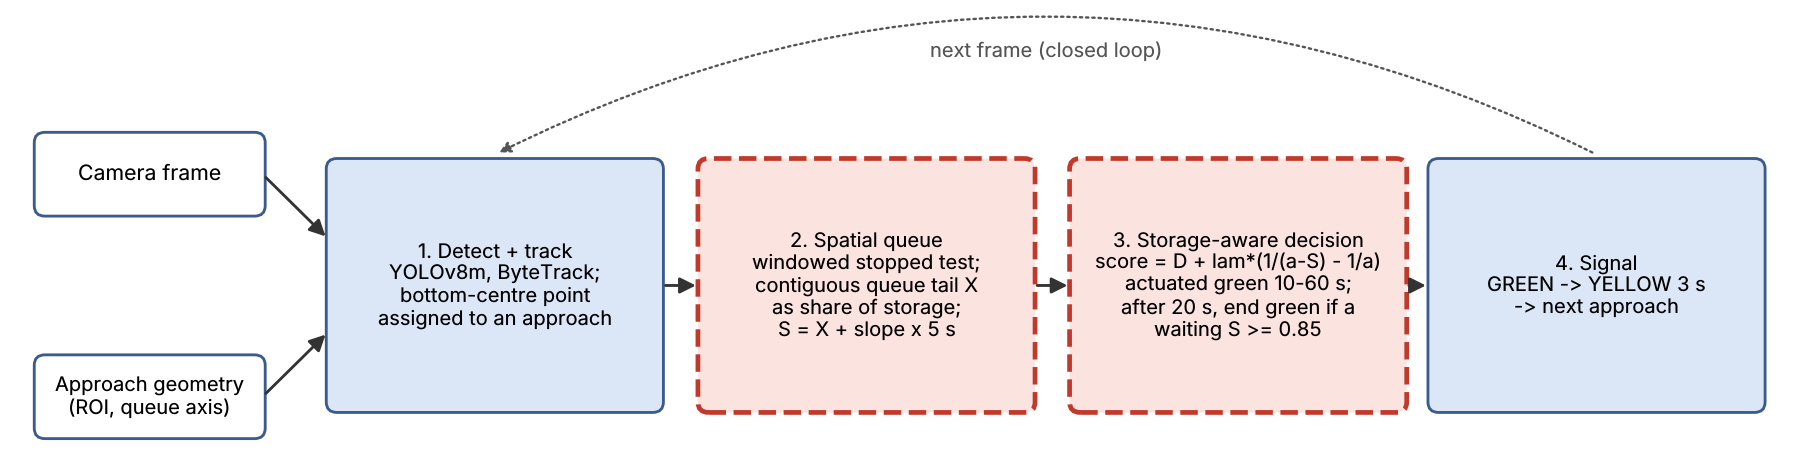
\includegraphics[width=0.92\textwidth]{fig_method_flow_crop.png}
\caption{Processing pipeline. The dashed blocks are the parts developed in this work.}
\label{fig:flow}
\end{figure*}

\subsection{Geometry}
For each approach we draw, once per camera, a region of interest over the inbound
lanes, a short strip behind the stop line, and a \emph{queue axis}: a polyline from the
stop line back along the lanes to the edge of the view. A vehicle is represented by the
bottom-centre of its box, the point where it meets the road surface. Its position along
the approach is the arc length of the projection of that point onto the axis, divided
by the axis length $L$:
\begin{equation}
p = \frac{\ell_k+\operatorname{clip}_{[0,L_k]}((\mathbf{r}-\mathbf{a}_k)\cdot\mathbf{u}_k)}{L},
\end{equation}
where $k$ is the nearest segment, $\ell_k$ its starting arc length, $L_k$ its length and $\mathbf{u}_k$ its unit direction; hence $p\in[0,1]$. No camera calibration is required. The price is that $p$ is a fraction of
the \emph{visible} approach and is not metric.

\subsection{Stopped test}
A tracked vehicle is stopped when its displacement over the last second, divided by its
box height $h$, is below a threshold:
\begin{equation}
\frac{\lVert \mathbf{r}_t-\mathbf{r}_{t-1\,\mathrm{s}}\rVert}{h\cdot 1\,\mathrm{s}} < 0.2 .
\end{equation}
Dividing by $h$ compensates perspective: a distant vehicle covers few pixels per second
even when moving. The one-second window averages out frame-to-frame box jitter. This is an image-space heuristic, not a calibrated speed in m/s.

\subsection{Queue tail and risk}
Stopped vehicles are sorted by $p$. The queue is the chain that starts inside the stop-line strip or within one gap allowance of the line, and continues while consecutive members are separated
by at most two vehicle lengths, the length being the extent of the box along the local
road direction, $|w u_x|+|h u_y|$. The queue tail $X$ is the position of the last member.
An isolated stopped detection further upstream cannot set $X$.

The trend of $X$ is fitted by least squares over 2.5\,s and extrapolated:
\begin{equation}
S=\operatorname{clip}_{[0,1]}\bigl(X+\dot X\cdot 5\,\mathrm{s}\bigr).
\end{equation}
$S$ is a local risk of exhausting the visible storage. It does not detect downstream
spillback.

For comparison we also compute the count measures of the base method: density
$D$ (PCE-weighted count in the region divided by its capacity) and a stop-line queue
$Q$ (count in the strip divided by its capacity), and a count forecast
$F=\operatorname{clip}(Q+\dot Q\cdot 3\,\mathrm{s})$. Once the strip is full, $Q=1$ and
$\dot Q=0$, so $F$ cannot indicate further growth; $X$ continues to change.

\subsection{Evaluation on footage}
We use three clips (107\,s, 240\,s, 240\,s; 30\,fps) of one intersection from the City
of Bellevue traffic video dataset~\cite{bellevue}. Table~\ref{tab:measure} uses cached YOLOv8n tracks to compare the initial implementation (stopped: less than 2\,px since the previous frame; tail: furthest
stopped vehicle) with the method above. The initial version registered 4.28 stop events
per vehicle and moved $X$ by more than 0.3 of the approach between consecutive frames in
up to 7.3\% of frames. With the robust stopped test alone, $X$ became almost always zero,
which revealed that the original regions did not isolate inbound lanes or define a stop
line. After redrawing the geometry, stop events fell to 0.76 per vehicle and large jumps
to at most 1.1\% of frames. With YOLOv8m the busy clip gives 0.74 stops per vehicle, and the two longer clips give 0.57 and 0.56. Fig.~\ref{fig:frame} shows one frame.

The footage is lightly loaded: the stop-line strip is full ($Q=1$) in at most 6\% of frames
on any approach. The saturation of $Q$ and $F$ described above is therefore a property
of the definitions that these clips rarely exercise, and it is examined in simulation
instead.

\begin{table}[t]
\caption{Measurement audit on the busy clip, YOLOv8n (jump: $X$ changes by more than 0.3 between frames)}
\label{tab:measure}
\centering
\setlength{\tabcolsep}{3pt}
\begin{tabular}{lccc}
\toprule
 & Initial & Robust & Robust test,\\
 &         & test   & new geometry\\
\midrule
Stops per vehicle & 4.28 & 0.46 & 0.76\\
North: $X>0$ / jump & 99\% / 7.3\% & 0.2\% / 0.06\% & 70\% / 0.06\%\\
South: $X>0$ / jump & 58\% / 3.0\% & 0\% / 0\% & 48\% / 1.1\%\\
West: $X>0$ / jump & 59\% / 4.8\% & 0.2\% / 0\% & 58\% / 0.5\%\\
\bottomrule
\end{tabular}
\end{table}

\begin{figure}[t]
\centering
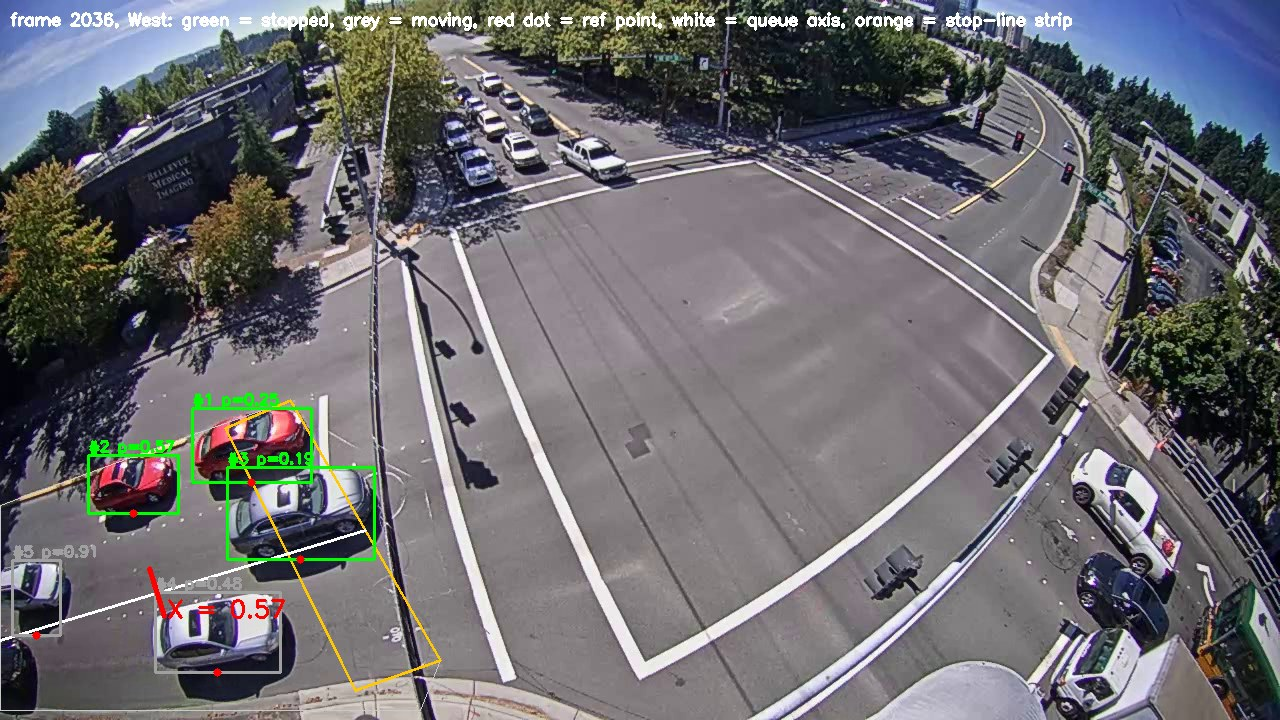
\includegraphics[width=\columnwidth]{frame_example.jpg}
\caption{West approach, frame 2036. Green boxes are stopped vehicles, grey are moving.
The chain of three stopped vehicles gives $X=0.57$ (red bar); a moving vehicle in the
adjacent lane is ignored.}
\label{fig:frame}
\end{figure}

Two limits remain. Detector recall falls with distance: on a test frame YOLOv8m found 4
of about 9 queued vehicles on the far north approach (YOLOv8n found 2), so $X$ is
underestimated there. And we have no hand-labelled queue ends, so accuracy is supported
by the proxies in Table~\ref{tab:measure} and visual inspection rather than by an error
against ground truth. The regions and axes are drawn by hand for this camera and would
have to be redrawn for another.

\section{Evaluation Method}
Recorded vehicles follow the signal that was filmed, so footage cannot show the effect of
a different controller. An earlier open-loop comparison on the clips reported 21\% more
vehicles served with the risk term; a control with the term set to zero and the same
weights reproduced the figure exactly, and the count of ``served'' vehicles was found to
measure overlap between the simulated green and the real one. Control is therefore
evaluated only in closed loop. The footage is still useful for one check that does not
depend on vehicle response: replaying identical tracks through each controller shows
which approach it would serve. On all three clips the controller with the risk term
serves the same approach as the controller without it at every green.

Several other extensions of the base controller were tried on the footage before the
closed-loop study and were not retained: a PCE-weighted queue (no effect, the traffic
is almost all cars), a count of vehicles stopped beyond the strip as a score term (no
consistent effect), a discharge-limited green time derived from the measured queue
(worse at this short region length), and a switching margin with a green-rate limit
(mixed). Ending the green as soon as the strip emptied also gave mixed results, because
greens were cut during discharge; requiring the strip to stay empty for a 2\,s passage
time removed the problem and is the actuated rule used below.

We use SUMO~\cite{sumo} through libsumo with a 0.5\,s step. The junction has four
two-lane approaches served one at a time with 3\,s yellow. A virtual camera computes
$D$, $Q$, $X$ and $S$ from simulated positions and speeds. It shares the predictor with the video pipeline but uses a fixed chain gap of 0.25 of link length and instantaneous speed below 0.2 vehicle lengths/s, rather than box-scaled gaps and temporal tracking. Optional noise drops up to 30\% of distant vehicles and adds 2\,m position jitter; speeds remain exact and tracking errors are not modelled. Arrivals are Poisson with 5\% heavy vehicles; each run has 1800\,s of demand and up to 900\,s for draining. Delay includes vehicles scheduled after 300\,s; blocked-entry time covers the full run, including warm-up and draining.

The primary measure is mean delay per vehicle (time loss plus the time waited to enter a
full link). The secondary measure is blocked-entry time: approach-seconds with pending SUMO insertions. It is a proxy for entry blockage and can include brief insertion conflicts rather than network spillback. All methods run on the same seeds; we report paired differences with 95\%
$t$-intervals over 20 seeds. Design choices were made on separate validation seeds and
the protocols were committed to the repository before the test seeds were run.

\section{Study 1: Queue Tail in the Selection Score}\label{sec:study1}
The first design adds the new measures to the score that ranks approaches:
\begin{equation}
\mathrm{score}_i=(1-\omega-\rho)\bigl[\alpha D_i+(1-\alpha)Q_i\bigr]+\omega F_i+\rho S_i ,
\end{equation}
with $\alpha=0.5$, $\omega=\rho=0.3$ for the proposed arm (S4). The ablation comprises
fixed-time (S0), actuated round-robin (A0), density only (S1), density and queue (S2),
plus count forecast (S3), S4, a null arm with S4's weights and $S\equiv 0$, and arms that
substitute $X$ or $S$ for $F$. Each score-based arm is run with band timing
(30/45/60\,s by score) and with actuated timing (10--60\,s, ended after the strip has been
empty for 2\,s), on nine demand scenarios from light to beyond capacity; one scenario
takes its per-approach demand shares from the vehicle counts measured on the footage.
Density is normalised either by the storage capacity of the approach, or by a small
constant so that it saturates as it does in the video configuration. The grid was run on
20 test seeds (100--119) after choices were fixed on seeds 0--3.

\begin{table}[t]
\caption{Study 1: mean delay per vehicle (s), 20 seeds, physical density normaliser}
\label{tab:study1}
\centering
\begin{tabular}{lccccc}
\toprule
 & S0 & S1 & A0 & S1 & S4\\
Scenario & fixed & bands & actuated & actuated & actuated\\
\midrule
Light & 43.5 & 45.5 & 20.3 & 20.3 & 20.2\\
Medium & 47.3 & 77.5 & 23.1 & 23.0 & 23.0\\
Heavy & 52.4 & 92.2 & 36.3 & 36.3 & 36.5\\
Unequal, over-sat. & 300.6 & 147.4 & 40.0 & 33.8 & 33.7\\
Over-saturated & 147.6 & 148.2 & 140.0 & 116.8 & 120.1\\
\bottomrule
\end{tabular}
\end{table}

Table~\ref{tab:study1} gives representative results. The timing rule dominates: actuated
timing roughly halves delay against fixed-time below capacity and reduces it from 300.6
to 33.8\,s under unequal over-saturated demand, whereas band timing is worse than
fixed-time in most scenarios because no green is shorter than 30\,s or ends early. With actuated timing and the saturating density normaliser, the paired difference S4$-$S3 is within $\pm0.1$\,s in eight scenarios and $+1.5\pm3.1$\,s in the ninth; none shows a significant improvement. A decision-level comparison on identical traffic found that adding $S$
changed the approach served in 1 of 40 runs. The conclusions are the same for both
density normalisers and with the camera noise model. Blocked-entry time is not reduced
either: in the over-saturated scenario with actuated timing it is 4143\,s for S0, 3138\,s for S1 and
$3251\pm317$\,s for S4.

Two mechanisms explain this. First, a decision is taken when a green ends; every other
approach has been red and is accumulating a queue, and the approach with the longest
queue is also the one with the most vehicles, so in these runs $X$ usually ranks approaches as $D$ already does. Second,
$X$ loses discrimination as queues approach the edge of the visible storage. Spatial information can
therefore only add something where a count does not already carry it: in the timing
decision, and relative to the storage of each approach.

\section{Study 2: Queue Tail as a Storage Limit}\label{sec:study2}
\subsection{Method}
The second design follows the formulation of~\cite{mohajerpoor2023} but replaces the
modelled queue position by the measured one and the cycle optimisation by a rule
evaluated every step. Selection uses the base density with one additional term,
\begin{equation}
\mathrm{score}_i = D_i+\lambda\left(\frac{1}{\alpha-S_i}-\frac{1}{\alpha}\right),
\qquad \lambda=1,\ \alpha=1.1 ,
\label{eq:barrier}
\end{equation}
where $D_i$ uses a common normaliser for all approaches (it is storage-blind, as in the
base method) and $S_i$ is relative to the approach's own storage. The term uses the dimensionless reciprocal form of~\cite{mohajerpoor2023}, evaluated at the projected queue fraction and shifted to vanish for an empty approach; it is 0.76 at $S=0.5$ and 9.09 at $S=1$. Green time is
actuated, with one addition (\emph{storage protection}): after 20\,s of green, the green
ends if a waiting approach $j$ has
\begin{equation}
S_j\ge\beta=0.85 \quad\text{and}\quad S_j>S_{\mathrm{active}} .
\label{eq:protect}
\end{equation}

\subsection{Design}
Two geometries are used: all approaches 150\,m, and a junction whose minor street
(east/west) is 60\,m. Total demand is 1200, 1800, 2400, 3000 or 3600\,veh/h, split
35/30/20/15\% between north, south, east and west. The methods are fixed-time (FT);
actuated round-robin that skips empty approaches (ACT); capacity-normalised pressure (CMP), checked every 5\,s after a 10\,s minimum green (60\,s maximum)~\cite{gregoire2015}; Raza-style density with bands (RAZA); and an
ablation of the proposed controller: density with actuated timing (RAZA-A), plus the
barrier of~\eqref{eq:barrier} (PROP-B), plus protection~\eqref{eq:protect} (PROP), and
PROP with $S$ computed from the number of stopped vehicles divided by storage capacity
instead of the measured tail (PROP-CNT). PROP is also run with the camera noise model.

The values of $\lambda$, $\beta$ and the 20\,s guard were chosen on validation seeds
0--9. Without a guard, protection halved blocked-entry time at 3000\,veh/h but
multiplied delay at 3600\,veh/h. Three guards were compared under a rule fixed in
advance (delay within 5\% of PROP-B in every heavy condition). None satisfied it; the
variant with the smallest worst-case increase was frozen, and the test below was run
once on seeds 200--219.

\subsection{Results}
\begin{table*}[t]
\caption{Study 2: mean delay per vehicle (s). Best exact-sensor result per column in bold.}
\label{tab:delay}
\centering
\begin{tabular}{lcccccccccc}
\toprule
 & \multicolumn{5}{c}{All approaches 150 m} & \multicolumn{5}{c}{Minor street 60 m}\\
\cmidrule(lr){2-6}\cmidrule(lr){7-11}
Method / demand (veh/h) & 1200 & 1800 & 2400 & 3000 & 3600 & 1200 & 1800 & 2400 & 3000 & 3600\\
\midrule
FT & 46.2 & 48.0 & 56.7 & 133.5 & 283.6 & 45.9 & 47.7 & 56.3 & 133.4 & 283.7\\
ACT & 20.9 & 24.5 & 30.5 & 45.5 & 99.9 & 20.4 & 24.0 & 30.0 & \best{45.6} & 105.5\\
CMP~\cite{gregoire2015} & \best{16.9} & \best{19.9} & \best{26.3} & 157.4 & 397.8 & \best{17.7} & \best{22.1} & 37.3 & 167.6 & 389.5\\
RAZA~\cite{raza2025} & 53.6 & 71.9 & 85.6 & 131.2 & 253.5 & 53.2 & 69.0 & 77.8 & 91.9 & 165.2\\
RAZA-A & 21.7 & 24.5 & 30.5 & 45.6 & 100.6 & 21.5 & 24.0 & 30.0 & 46.1 & 108.5\\
PROP-B & 19.2 & 23.5 & 29.3 & 45.1 & \best{97.1} & 19.2 & 23.0 & 29.4 & 46.1 & \best{103.7}\\
PROP & 19.2 & 23.5 & 29.3 & \best{44.2} & 190.8 & 19.2 & 23.0 & 29.1 & 46.4 & 186.2\\
PROP-CNT & 19.2 & 23.1 & 29.3 & 44.4 & 142.8 & 18.9 & 22.7 & \best{28.9} & 46.5 & 156.3\\
\midrule
PROP, camera noise & 19.8 & 23.3 & 29.1 & 44.1 & 189.2 & 20.0 & 23.9 & 29.3 & 53.7 & 196.7\\
\bottomrule
\end{tabular}
\end{table*}

\begin{table}[t]
\caption{Study 2: blocked-entry time (s)}
\label{tab:spill}
\centering
\setlength{\tabcolsep}{4pt}
\begin{tabular}{lcccccc}
\toprule
 & \multicolumn{3}{c}{All 150 m} & \multicolumn{3}{c}{Minor 60 m}\\
\cmidrule(lr){2-4}\cmidrule(lr){5-7}
Method & 2400 & 3000 & 3600 & 2400 & 3000 & 3600\\
\midrule
FT & 164 & 2172 & 4135 & 652 & 3093 & 5441\\
ACT & 7 & 120 & 2136 & 97 & 945 & \best{4097}\\
CMP & \best{7} & 2442 & 6164 & \best{14} & 3343 & 6495\\
RAZA & 785 & 2366 & 4195 & 1957 & 3347 & 5361\\
RAZA-A & 7 & 132 & 2153 & 103 & 983 & 4160\\
PROP-B & 7 & 114 & \best{2105} & 92 & 982 & 4161\\
PROP & 7 & \best{89} & 3193 & 79 & \best{753} & 4326\\
PROP-CNT & 7 & 104 & 2718 & 81 & 869 & 4365\\
\midrule
PROP, noise & 7 & 81 & 3143 & 92 & 922 & 4340\\
\bottomrule
\end{tabular}
\end{table}

\begin{figure*}[t]
\centering
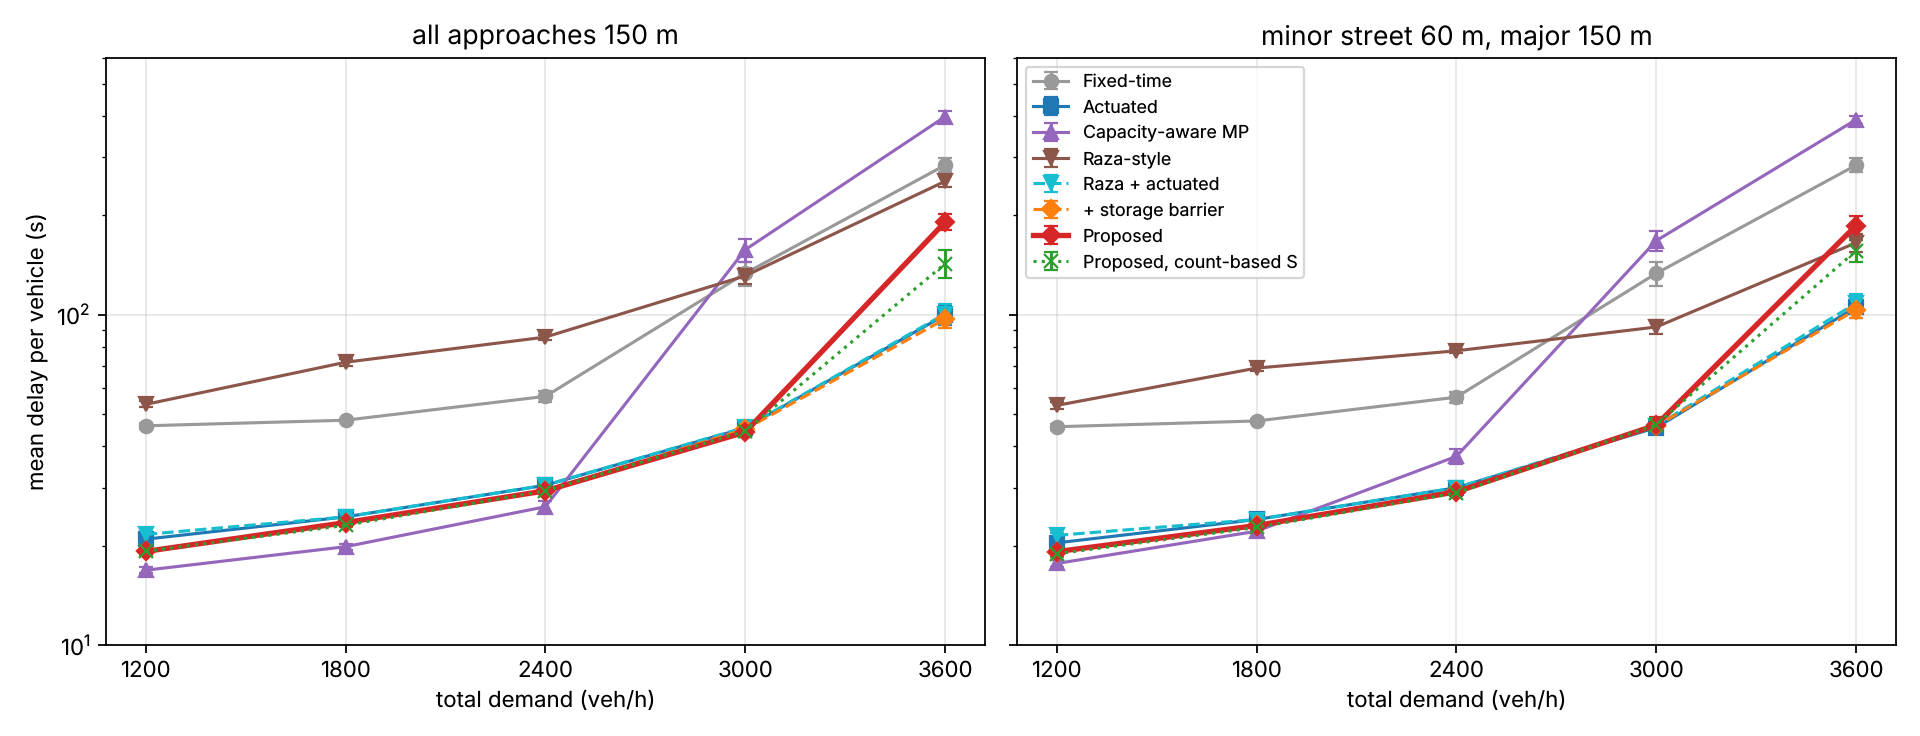
\includegraphics[width=0.49\textwidth]{fig_s2_delay.png}\hfill
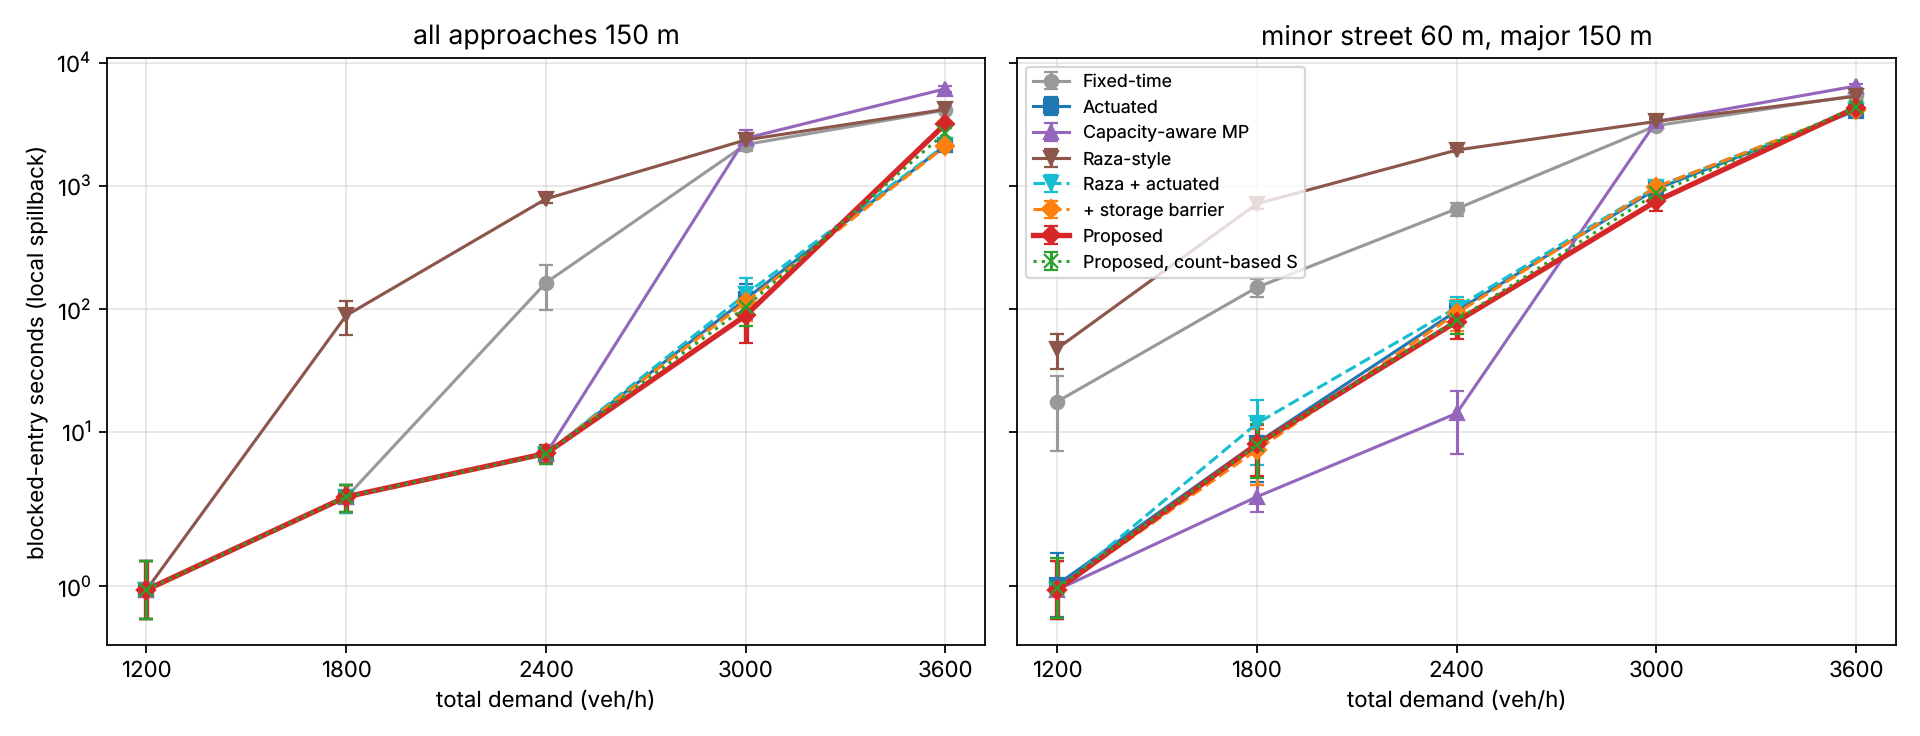
\includegraphics[width=0.49\textwidth]{fig_s2_spillback.png}
\caption{Study 2: mean delay (left pair) and blocked-entry time (right pair) against
total demand for the two geometries. Bars are 95\% intervals over 20 seeds.}
\label{fig:curves}
\end{figure*}

Tables~\ref{tab:delay} and~\ref{tab:spill} and Fig.~\ref{fig:curves} give the results;
Table~\ref{tab:paired} lists the pre-specified paired comparisons.

\emph{Against the base method.} PROP has 34--87\,s less delay than RAZA in nine of the
ten conditions. The ablation attributes most of this to actuated timing: RAZA-A is
within 1--2.5\,s of PROP below capacity. At 3600\,veh/h on the short-minor geometry RAZA
is better than PROP by $21.0\pm10.5$\,s.

\emph{Against actuated control.} Up to 2400\,veh/h PROP has 0.9--1.7\,s less delay than
ACT. This difference cannot be attributed to the storage term alone, because PROP also
selects by score and never serves the same approach twice in succession, and no arm
separates these effects. At 3000\,veh/h, near capacity, PROP reduces blocked-entry time
by $31.9\pm20.6$\,s ($-26\%$) on the uniform geometry and by $191.8\pm73.3$\,s ($-20\%$)
on the short-minor geometry. Delay is $1.3\pm0.9$\,s lower on the uniform geometry and $0.8\pm1.6$\,s higher on the short-minor geometry; only the former excludes zero.

\emph{Effect of protection and of the measurement.} Relative to PROP-B, protection alone
reduces blocked-entry time at 3000\,veh/h by $25.3\pm19.1$\,s and $229.2\pm70.3$\,s on the
two geometries. Relative to PROP-CNT, the measured tail reduces it by a further
$115.4\pm81.2$\,s on the short-minor geometry; At 3600\,veh/h the count variant instead has less delay on both geometries.

\emph{Beyond capacity.} At 3600\,veh/h PROP is worse than ACT by $90.9\pm9.8$\,s and
$80.7\pm8.1$\,s of delay. Every approach is then close to full, some waiting approach
always satisfies~\eqref{eq:protect}, greens are cut repeatedly, and each change costs a
yellow interval, which lowers capacity further. This is the queue-formation regime in
which~\cite{mohajerpoor2023} relax the constraint.

\emph{Other observations.} CMP has the lowest delay at light demand (about 2\,s below
PROP) and the highest at 3000\,veh/h and above, under this implementation; this does not establish a general weakness of pressure control.
With camera noise PROP has similar mean delay up to 2400\,veh/h; at 3000\,veh/h on the short-minor
geometry blocked-entry time rises from 753 to 922\,s and delay from 46.4 to 53.7\,s, so
most of the benefit over ACT is lost.

\begin{table}[t]
\caption{Study 2: paired differences, PROP minus reference (mean $\pm$ 95\% CI). Negative favours PROP.}
\label{tab:paired}
\centering
\setlength{\tabcolsep}{3pt}
\begin{tabular}{llcc}
\toprule
Reference & Condition & $\Delta$ delay (s) & $\Delta$ blocked (s)\\
\midrule
RAZA & uniform 3000 & $-87.0\pm6.5$ & $-2277\pm123$\\
ACT & uniform 3000 & $-1.3\pm0.9$ & $-31.9\pm20.6$\\
ACT & short-minor 3000 & $+0.8\pm1.6$ & $-191.8\pm73.3$\\
PROP-B & uniform 3000 & $-0.9\pm0.9$ & $-25.3\pm19.1$\\
PROP-B & short-minor 3000 & $+0.3\pm1.6$ & $-229.2\pm70.3$\\
PROP-CNT & short-minor 3000 & $-0.1\pm1.9$ & $-115.4\pm81.2$\\
ACT & uniform 3600 & $+90.9\pm9.8$ & $+1057\pm181$\\
ACT & short-minor 3600 & $+80.7\pm8.1$ & $+229\pm137$\\
\bottomrule
\end{tabular}
\end{table}

\section{Discussion and Limitations}
The spatial measure had no significant delay benefit in the selection score and a measurable effect as a
timing constraint. In the score it is redundant with the count at the moment decisions
are taken. As a constraint it acts between decisions and relative to each approach's
storage, where the count carries no information. The comparison with PROP-CNT suggests
the measured position matters when queues are long relative to the link, without establishing superiority across demand regimes.

Several limitations qualify these results. (i) The measurement is a fraction of the
visible approach, is not metric, and underestimates queues on distant approaches where
detections are missed; its accuracy has not been scored against hand-labelled queue ends.
(ii) The control results come from simulation of a single isolated junction. An isolated
junction charges spillback only as waiting time, whereas in a network a blocked link
obstructs the upstream junction, so network effects remain to be measured on a corridor. (iii) The protection rule has no
notion of regime; beyond capacity it is harmful. Detecting that all approaches are near
full and relaxing $\beta$, as in~\cite{mohajerpoor2023}, is the natural correction.
(iv) Thresholds and weights were set by hand or on a small validation set. (v) The
footage is three short clips (587\,s in total) of one junction in daylight, and the
simulated junction has straight-through movements and Poisson arrivals only. (vi) Eight fixed-time runs at 3600\,veh/h have unfinished vehicles at the drain limit; their recorded losses are censored. (vii) The simplified sensor and pressure baseline limit transfer to deployed systems. (viii) The base controller is Raza-style rather than a reproduction: bands are 30/45/60\,s instead of
40/60/120\,s and lane-priority weights are not used, because the camera's approaches are
not separated by turning movement.

\section{Conclusion}
We presented a calibration-free method to measure the queue tail from a traffic camera
and tested two ways of using it for signal control. As an additional ranking term it rarely changes choices and gives no significant delay improvement in these tests. As a
storage limit on green time it reduces local spillback by 20--26\% near capacity without an observed delay penalty, improves on a count-based equivalent when storage is short, and fails
beyond capacity. Future work is a regime-aware version of the rule, a metric queue
position through a ground-plane homography, better recall on distant approaches, and a
multi-junction evaluation.

\section*{Acknowledgment}
The video data are from the City of Bellevue traffic video dataset. AI-assisted tools were
used in developing the software, running the experiments and preparing the text; the authors are responsible for the content.

\begin{thebibliography}{00}
\bibitem{raza2025} M. Raza \emph{et al.}, ``An edge-deployed real-time adaptive traffic
light control system using YOLO-based vehicle detection and PCE-aware density
estimation,'' \emph{IEEE Access}, vol. 13, pp. 153586--153613, 2025, doi: 10.1109/ACCESS.2025.3602844.
\bibitem{mohajerpoor2023} R. Mohajerpoor, C. Cai, and M. Ramezani, ``Optimal traffic
signal control of isolated oversaturated intersections using predicted demand,''
\emph{IEEE Trans. Intell. Transp. Syst.}, vol. 24, no. 1, pp. 815--826, Jan. 2023, doi: 10.1109/TITS.2022.3209606.
\bibitem{li2025} C. Li, Y. Lu, and H. Wang, ``A multi-objective model for traffic signal
coordination control with queue profile estimation,'' \emph{IEEE Trans. Intell. Transp.
Syst.}, vol. 26, no. 12, pp. 23389--23406, 2025, doi: 10.1109/TITS.2025.3616119.
\bibitem{wei2025} L. Wei, K. Ampountolas, A. Hirrle, and M. Wang, ``Hierarchical predictive control
of network traffic signals using link transmission model with queue dynamics,''
\emph{IEEE Trans. Intell. Transp. Syst.}, vol. 26, no. 10, pp. 16391--16404, 2025, doi: 10.1109/TITS.2025.3568869.
\bibitem{stm2015} T. Urbanik \emph{et al.}, \emph{Signal Timing Manual}, 2nd ed., NCHRP
Report 812. Washington, DC, USA: Transportation Research Board, 2015.
\bibitem{varaiya2013} P. Varaiya, ``Max pressure control of a network of signalized
intersections,'' \emph{Transp. Res. Part C}, vol. 36, pp. 177--195, 2013.
\bibitem{gregoire2015} J. Gregoire, X. Qian, E. Frazzoli, A. de La Fortelle, and T.
Wongpiromsarn, ``Capacity-aware backpressure traffic signal control,'' \emph{IEEE Trans.
Control Netw. Syst.}, vol. 2, no. 2, pp. 164--173, 2015.
\bibitem{yolov8} G. Jocher, A. Chaurasia, and J. Qiu, ``Ultralytics YOLOv8,'' 2023.
[Online]. Available: https://github.com/ultralytics/ultralytics
\bibitem{bytetrack} Y. Zhang \emph{et al.}, ``ByteTrack: Multi-object tracking by
associating every detection box,'' in \emph{Proc. ECCV}, 2022.
\bibitem{sumo} P. A. Lopez \emph{et al.}, ``Microscopic traffic simulation using SUMO,''
in \emph{Proc. IEEE ITSC}, 2018.
\bibitem{bellevue} City of Bellevue, ``Traffic video dataset.'' [Online]. Available:
https://github.com/City-of-Bellevue/TrafficVideoDataset
\end{thebibliography}

\end{document}
